FET, field effekt transistor, er en type transistor.
En FET kalles en \emph{unipolar} komponent fordi de har én type bærere.
Ladningstransporten skjer ved majoritetsbærere.

Fordeler:
\begin{itemize}
\item Spenningsregulert: Kan anses som en spenningskontrollert strømkilde.
\item Veldig stor inngangsmotstand. Som gjør den energieffektiv.
\end{itemize}

Ulemper:
\begin{itemize}
\item Lav transkonduktans. Som gir liten forsterkning.
\end{itemize}



\subsubsection{To typer}
Field effekt transistorer kommer i 2 typer
\\
\paragraph{JFET: Junction Field Effekt Transistor} \mbox{} \\
JFET er den første typen FET som ble laget.
De deles igjen i to typer, n-channel og p-channel, avhengig av hva slags doping
som er brukt på den innerste halvlederen.
\\
\paragraph{MOSFET: Metall Oksyd Semiconductor FET} \mbox{} \\
MOSFET er en nyere teknologi enn JFET.
Kommer også som n-channel eller p-channel, men kommer i tillegg som en av:\\
E-MOSFET - Enhancement mode MOSFET (er på med tilstrekkelig spenning på gate) \\
D-MOSFET - Depletion mode MOSFET (er på uten spenning på gate)



\subsubsection{JFET}
Når vi har sett på transistorer har vi sett på de 3 terminalene Base, Collector
og Emitter.
For helligdom og mystikk kalles de i FET-sammenheng for Gate, Drain og Source.
\\\\
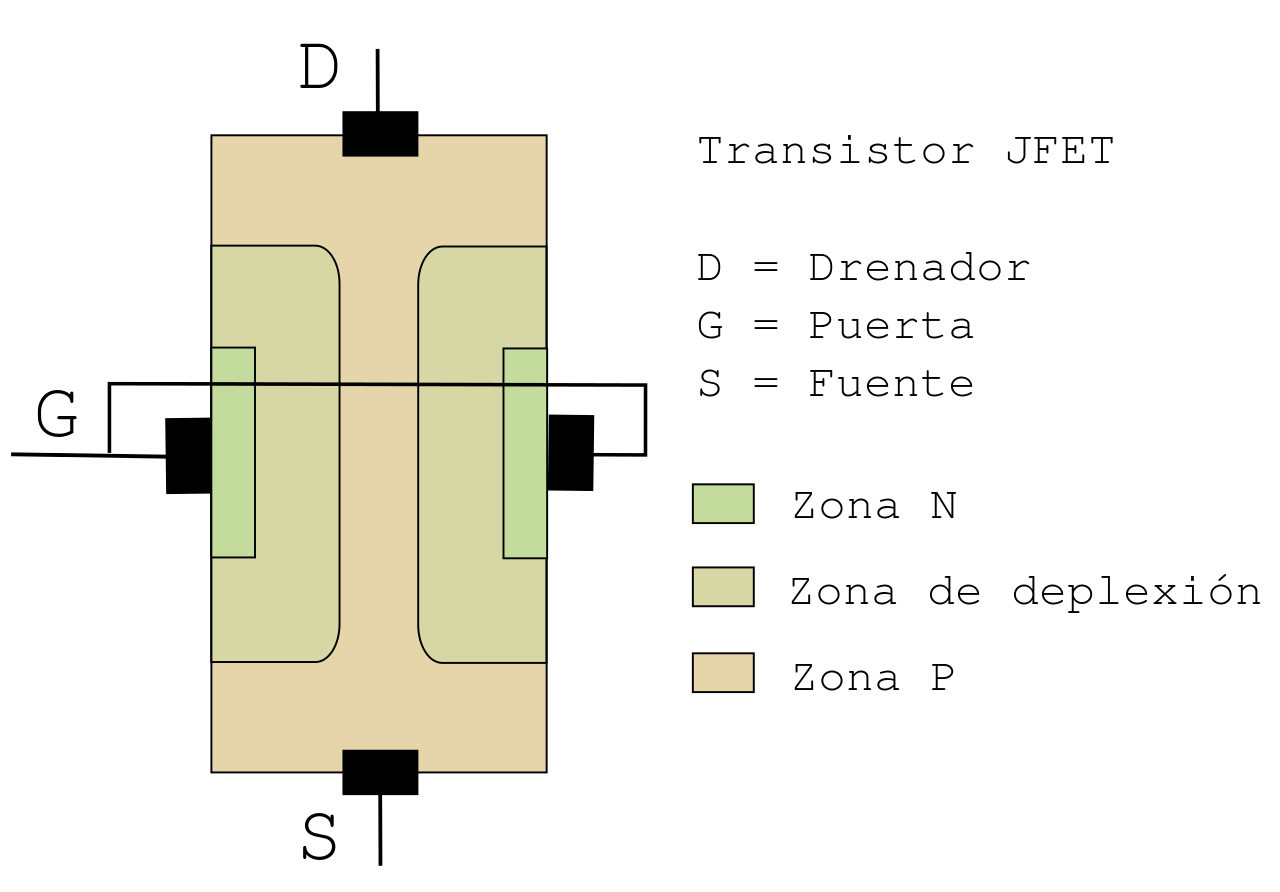
\includegraphics[width=\textwidth]{./img/jfet}
\\\\
Gate er koblet på n-dopet materiale, vi ser sperresjikte i lysegrønn og
i midten er et p-dopet materiale.
Dette bildet er et eksempel på p-channel JFET.
Hvis n og p materialene var byttet om ville det være en n-channel.


\subsubsection{MOSFET}
\paragraph{D-MOSFET} \mbox{} \\
D-MOSFET kalles depletion (nedbryting) mosfet fordi det n-dopede materialet blir
positivt ladet og derfor \emph{brytes ned}.
Se på den visuelle likheten mellom dmosfet og emosfet så forstår du hva
jeg mener.
\\\\
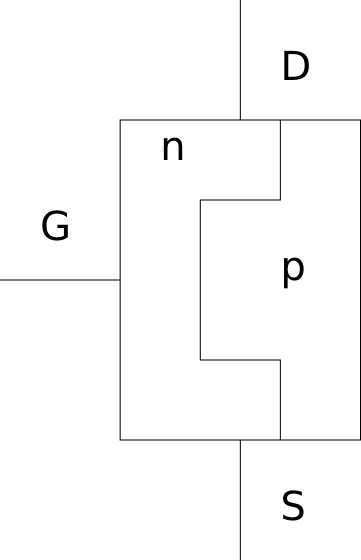
\includegraphics[width=0.5\textwidth]{./img/dmosfet}
\\\\
Mellom Gate og n-type er det en isolator som ikke er tegnet i inn.
\\\\
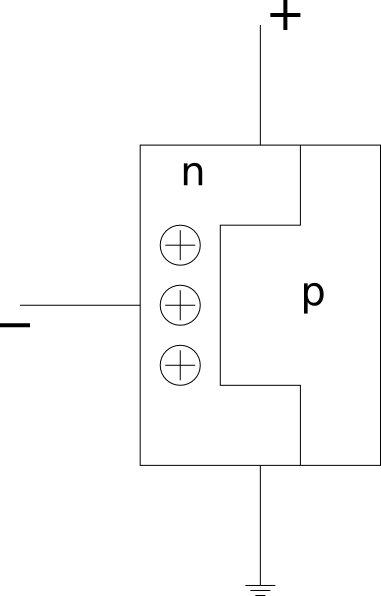
\includegraphics[width=0.5\textwidth]{./img/dmosfet-depleted}
\\\\
Her ser vi at n-materialet har mistet elektroner og er derfor brutt
ned (depleted).



\paragraph{E-MOSFET} \mbox{} \\
Enhancement (legge til) mosfet fungerer omtrent motsatt fra en dmosfet.
Istedenfor at n-området brytes i to, er den allerede brutt i to, men det kan
fylles igjen.
\\\\
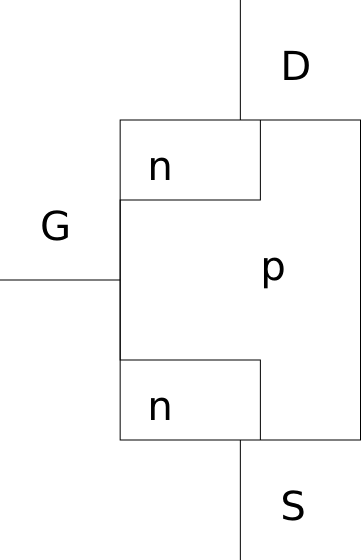
\includegraphics[width=0.5\textwidth]{./img/emosfet}


\subsubsection{CMOS}
CMOS er en teknologi som brukes i konstruksjon av integrerte kretser.
Navnet er et akronym for Complementary Metal Oxide Semiconductor.
En cmos-krets består av mosfet-transistorer.
Teknologien brukes i bl.a. mikroprosessorer, mikrokontroller, portkretser, SRAM.
\\\\
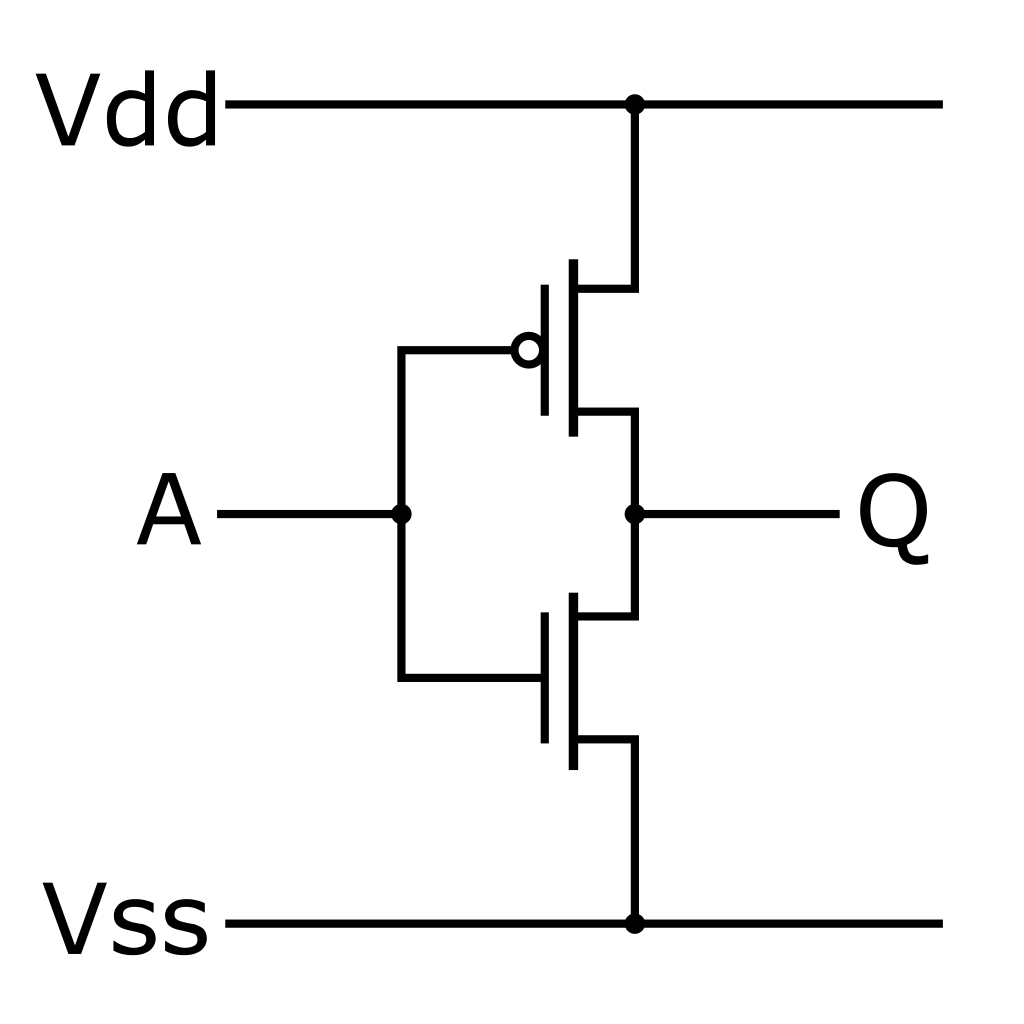
\includegraphics[width=0.5\textwidth]{./img/cmos-inverter}

